\subsection{Predikce}
Jakmile máme adekvátní model, můžeme ho použít pro bodové a intervalové predikce jako u jednorozměrné regrese

\textbf{ a) predikce} $ \E [ \textbf{Y}_{\textbf{x}} ] $

Nechť $ \textbf{x}_0 = ( 1, x_{0,1} , \dots , x_{0,m} )^{T} $ je nový bod proměnné $ \textbf{x} $ bodový odhad $ \E [ \textbf{Y}_{\textbf{x}_0} ] $ je roven 
$$
 \widehat{y}_{\textbf{x}_0} = \widehat{\beta}_0 + \sum_{j=1}^{m} x_{0,j} \widehat{\beta}_j = \textbf{x}_0^{T} \widehat{\beta} 
$$

tzn. $ \D [ \widehat{\textbf{Y}}_{\textbf{x}_0} ] = \textbf{x}_0^{T} \cdot \D [ \widehat{\beta} ] \cdot \textbf{x}_0 = \sigma^{2} \textbf{x}_0^{T}( \X ^{T} \X )^{-1} \textbf{x}_0 $ a může být odhadnut pomocí \\
$
 \widehat{\sigma}^{2}(\widehat{\textbf{Y}}_{\textbf{x}_0}) = s_n^2 [ \textbf{x}_0^{T}( \X ^{T} \X )^{-1} \textbf{x}_0 ]  $ (rozptyl predikce). Speciálně pokud $ \textbf{x}_0^{T} = \textbf{x}_i^{T} $ ( $ i $-tý řádek matice $ \X $)
 $$
  \widehat{\sigma}^{2}(\widehat{\textbf{Y}}_{\textbf{x}_i}) = s_n^2 [ \textbf{x}_i^{T}( \X ^{T} \X )^{-1} \textbf{x}_i ] = s_n^2 h_{ii} \quad \text{kde} \quad h_{ii} = (\text{H})_{ii} \quad \text{a} \quad \text{H} = \X (\X ^{T}  \X )^{-1} \X ^{T}.
 $$
Pro normální chyby lze odvodit interval spolehlivosti pro $ \E [\textbf{Y}_{\textbf{x}_0}] = \gamma_{\textbf{x}_0} $, protože $ \widehat{\textbf{Y}}_{\textbf{x}_0} $ je LK náhodné veličiny s vícerozměrným normálním rozdělením, má normální rozdělení se \\ $ \E [\widehat{\textbf{Y}}_{\textbf{x}_0}] = \gamma_{\textbf{x}_0} = \textbf{x}_0^{T} \beta $ a $ \D [ \widehat{\textbf{Y}}_{\textbf{x}_0} ] = \sigma^{2} \textbf{x}_0^{T}( \X ^{T} \X )^{-1} \textbf{x}_0 $
tzn.
$$
\frac{\widehat{\textbf{Y}}_{\textbf{x}_0} - \gamma_{\textbf{x}_0}}{\sigma \sqrt{\textbf{x}_0^{T}( \X ^{T} \X )^{-1} \textbf{x}_0}} \sim \text{N}(0,1) 
$$
a díky nezávislosti $ \widehat{\beta} $ a $ s_n^2 $
$$
 \frac{\widehat{\textbf{Y}}_{\textbf{x}_0} - \gamma_{\textbf{x}_0}}{s_n \sqrt{\textbf{x}_0^{T}( \X ^{T} \X )^{-1} \textbf{x}_0}} \sim \text{t}(n-m-1) \quad \Rightarrow \quad 100(1 - \alpha) \% \quad \text{IS pro } \gamma_{\textbf{x}_0}:
$$
$$
   ( \widehat{\textbf{Y}}_{\textbf{x}_0} \pm \text{t}_{1-\frac{\alpha}{2}}(n-m-1) \cdot s_n \sqrt{\textbf{x}_0^{T}( \X ^{T} \X )^{-1} \textbf{x}_0})
$$

\textbf{ b) interval predikce pro } $ \textbf{Y}_{\textbf{x}_0} $ 

Bodový odhad je opět $ \widehat{\textbf{Y}}_{\textbf{x}_0} $, pokud $ \textbf{Y}_{\textbf{x}_0} $  je skutečná hodnota $ \textbf{Y}_{\textbf{x}} $ v bodě $ \textbf{x} = \textbf{x}_0 $, potom $ \textbf{Y}_{\textbf{x}_0} $ a $ \widehat{\textbf{Y}}_{\textbf{x}_0} $ budou nezávislé za předpokladu, že pozorování $ \textbf{Y}_{\textbf{x}_0} , \text{Y}_1 , \dots , \text{Y}_n $ jsou nezávislé (což předpokládáme), 
potom 
$$
\D [ \widehat{\textbf{Y}}_{\textbf{x}_0} - \textbf{Y}_{\textbf{x}_0} ] = \D [ \widehat{\textbf{Y}}_{\textbf{x}_0} ] - \D [ \textbf{Y}_{\textbf{x}_0} ] = \sigma^{2}(1+ \textbf{x}_0^{T}( \X ^{T} \X )^{-1} \textbf{x}_0 ),
$$
takže
$$
\frac{\widehat{\textbf{Y}}_{\textbf{x}_0} - \textbf{Y}_{\textbf{x}_0}}{\sigma \sqrt{1+ \textbf{x}_0^{T}( \X ^{T} \X )^{-1} \textbf{x}_0 }} \sim \text{N}(0,1) \quad \text{a} \quad \frac{\widehat{\textbf{Y}}_{\textbf{x}_0} - \textbf{Y}_{\textbf{x}_0}}{s_n \sqrt{1+ \textbf{x}_0^{T}( \X ^{T} \X )^{-1} \textbf{x}_0 }} \sim \text{t}(n-m-1)
$$
za předpokladu normality chyb. \\
$ 100(1-\alpha) \% $ IP pro $ \textbf{Y}_{\textbf{x}_0} $ tedy je
$$
 (\widehat{\textbf{Y}}_{\textbf{x}_0} \pm \text{t}_{1 - \frac{\alpha}{2}}(n-m-1) \cdot s_n \sqrt{1+ \textbf{x}_0^{T}( \X ^{T} \X )^{-1} \textbf{x}_0 }) 
$$
\begin{example}
	\begin{remark}[Extrapolace]
	    \begin{itemize}
	    \item U jednoduché LR kvalitu predikce závisela na vzdálenosti $ x_0 $ od $ \overline{x} $.
	    \item Je třeba si dát pozor na predikce mimo $ [x_{min},x_{max}] $.
	    \item Podobné závěry platí i pro vícerozměrnou LR.
	    \item Protože rozptyl predikce je úměrný $ \textbf{x}_0^{T}( \X ^{T} \X )^{-1} \textbf{x}_0 $, v bodech s velkými hodnotami této veličiny nebude predikce spolehlivá.
	    \item Speciálně pokud $ \textbf{x}_i^T $ jsou pozorovaná data, můžeme očekávat, že body s nejvyššími hodnotami $ \textbf{x}_0^{T}( \X ^{T} \X )^{-1} \textbf{x}_0 = h_{ii} $ budou na hranici množiny, kde je predikce spolehlivá.
	    \end{itemize}
	    tzn., že vnitřek elipsoidu 
	    $$
	       \textbf{x}_0^{T}( \X ^{T} \X )^{-1} \textbf{x}_0 \leq     \max_{1 \leq j \leq n} h_{ii}
	    $$
	    může být považován za přípustný obor predikce
	    \begin{figure}[h]
	\centering
    \begin{tikzpicture}
    \node[inner sep=0pt] (pic) at (0,0)
    {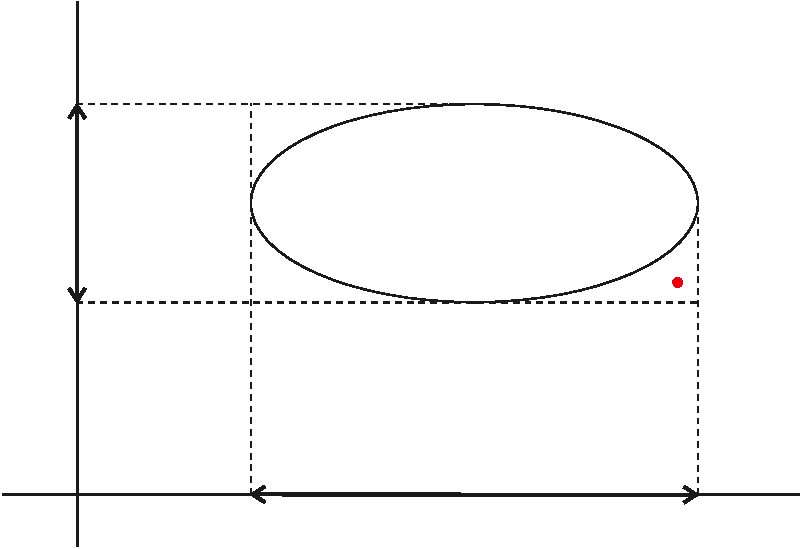
\includegraphics[width=13cm]{pictures/picture_3_F.pdf}};
    \draw [color=red](5.0,0.0) node[anchor=north west] {$(x_{01},x_{02})$};
    \draw [color=black](-5.9,4.2) node[anchor=north west] {$ x_2 $};
    \draw [color=black](5.5,-3.7) node[anchor=north west] {$ x_1 $};
     \draw [color=black](-1.0,1.4) node[anchor=north west] {$ \text{společný obor dat } (x_1, x_2) $};
     \draw [color=black](-0.0,-3.6) node[anchor=north west] {$ \text{obor hodnot } x_1 $};
     \draw [color=black](-8.4,1.4) node[anchor=north west] {$ \text{obor hodnot } x_2 $};
    \end{tikzpicture}
    \caption{ $(x_{01},x_{02})$ leží uvnitř oboru hodnot pro obě $ x_1 $ i $ x_2 $ ale vně společného oboru původních dat.}
\end{figure}
	\end{remark}
\end{example}